\documentclass[10pt]{article}
\usepackage[T1]{fontenc}

% Document Details
\newcommand{\CLASS}{AMATH 561}
\newcommand{\assigmentnum}{Assignment 1}

\usepackage[margin = 1.15in, top = 1.25in, bottom = 1.in]{geometry}

\usepackage{titling}
\setlength{\droptitle}{-6em}   % This is your set screw
\date{}
\renewcommand{\maketitle}{
	\clearpage
	\begingroup  
	\centering
	\LARGE \sffamily\textbf{\CLASS} \Large \assigmentnum\\[.8em]
	\large Tyler Chen\\[1em]
	\endgroup
	\thispagestyle{empty}
}
 % Title Styling
\usepackage{tocloft}
\renewcommand{\cfttoctitlefont}{\Large\sffamily\bfseries}
\renewcommand{\cftsecfont}{\normalfont\sffamily\bfseries}
\renewcommand{\cftsubsecfont}{\normalfont\sffamily}
\renewcommand{\cftsubsubsecfont}{\normalfont\sffamily}

\makeatletter
\let\oldl@section\l@section
\def\l@section#1#2{\oldl@section{#1}{\sffamily\bfseries#2}}

\let\oldl@subsection\l@subsection
\def\l@subsection#1#2{\oldl@subsection{#1}{\sffamily#2}}

\let\oldl@subsubsection\l@subsubsection
\def\l@subsubsection#1#2{\oldl@subsubsection{#1}{\sffamily#2}}
 % General Styling


\usepackage{enumitem}

% Figures
\usepackage{subcaption}

% TikZ and Graphics
\usepackage{tikz, pgfplots}
\pgfplotsset{compat=1.12}
\usetikzlibrary{patterns,arrows}
\usepgfplotslibrary{fillbetween}

\usepackage{pdfpages}
\usepackage{adjustbox}

\usepackage{lscape}
\usepackage{titling}
\usepackage[]{hyperref}


% Header Styling
\usepackage{fancyhdr}
\pagestyle{fancy}
\lhead{\sffamily \CLASS}
\rhead{\sffamily Chen \textbf{\thepage}}
\cfoot{}

% Paragraph Styling
\setlength{\columnsep}{1cm}
\setlength{\parindent}{0pt}
\setlength{\parskip}{5pt}
\renewcommand{\baselinestretch}{1}

% TOC Styling
\usepackage{tocloft}
\iffalse
\renewcommand{\cftsecleader}{\cftdotfill{\cftdotsep}}

\renewcommand\cftchapafterpnum{\vskip6pt}
\renewcommand\cftsecafterpnum{\vskip10pt}
\renewcommand\cftsubsecafterpnum{\vskip6pt}

% Adjust sectional unit title fonts in ToC
\renewcommand{\cftchapfont}{\sffamily}
\renewcommand{\cftsecfont}{\bfseries\sffamily}
\renewcommand{\cftsecnumwidth}{2em}
\renewcommand{\cftsubsecfont}{\sffamily}
\renewcommand{\cfttoctitlefont}{\hfill\bfseries\sffamily\MakeUppercase}
\renewcommand{\cftaftertoctitle}{\hfill}

\renewcommand{\cftchappagefont}{\sffamily}
\renewcommand{\cftsecpagefont}{\bfseries\sffamily}
\renewcommand{\cftsubsecpagefont}{\sffamily}
\fi
 % General Styling
% Code Display Setup
\usepackage{listings,lstautogobble}
\usepackage{lipsum}
\usepackage{courier}
\usepackage{catchfilebetweentags}

\lstset{
	basicstyle=\small\ttfamily,
	breaklines=true, 
	frame = single,
	rangeprefix=,
	rangesuffix=,
	includerangemarker=false,
	autogobble = true
}


\usepackage{algorithmicx}
\usepackage{algpseudocode}

\newcommand{\To}{\textbf{to}~}
\newcommand{\DownTo}{\textbf{downto}~}
\renewcommand{\algorithmicdo}{\hspace{-.2em}\textbf{:}}
 % Code Display Setup
% AMS MATH Styling
\usepackage{amsmath, amssymb}
\newcommand{\qed}{\hfill\(\square\)}

%\newtheorem*{lemma}{Lemma} 
%\newtheorem*{theorem}{Theorem}
%\newtheorem*{definition}{Definition}
%\newtheorem*{prop}{Proposition}
%\renewenvironment{proof}{{\bfseries Proof.}}{}


% mathcal
\newcommand{\cA}{\ensuremath{\mathcal{A}}}
\newcommand{\cB}{\ensuremath{\mathcal{B}}}
\newcommand{\cC}{\ensuremath{\mathcal{C}}}
\newcommand{\cD}{\ensuremath{\mathcal{D}}}
\newcommand{\cE}{\ensuremath{\mathcal{E}}}
\newcommand{\cF}{\ensuremath{\mathcal{F}}}
\newcommand{\cG}{\ensuremath{\mathcal{G}}}
\newcommand{\cH}{\ensuremath{\mathcal{H}}}
\newcommand{\cI}{\ensuremath{\mathcal{I}}}
\newcommand{\cJ}{\ensuremath{\mathcal{J}}}
\newcommand{\cK}{\ensuremath{\mathcal{K}}}
\newcommand{\cL}{\ensuremath{\mathcal{L}}}
\newcommand{\cM}{\ensuremath{\mathcal{M}}}
\newcommand{\cN}{\ensuremath{\mathcal{N}}}
\newcommand{\cO}{\ensuremath{\mathcal{O}}}
\newcommand{\cP}{\ensuremath{\mathcal{P}}}
\newcommand{\cQ}{\ensuremath{\mathcal{Q}}}
\newcommand{\cR}{\ensuremath{\mathcal{R}}}
\newcommand{\cS}{\ensuremath{\mathcal{S}}}
\newcommand{\cT}{\ensuremath{\mathcal{T}}}
\newcommand{\cU}{\ensuremath{\mathcal{U}}}
\newcommand{\cV}{\ensuremath{\mathcal{V}}}
\newcommand{\cW}{\ensuremath{\mathcal{W}}}
\newcommand{\cX}{\ensuremath{\mathcal{X}}}
\newcommand{\cY}{\ensuremath{\mathcal{Y}}}
\newcommand{\cZ}{\ensuremath{\mathcal{Z}}}

% mathbb
\usepackage{bbm}
\newcommand{\bOne}{\ensuremath{\mathbbm{1}}}

\newcommand{\bA}{\ensuremath{\mathbb{A}}}
\newcommand{\bB}{\ensuremath{\mathbb{B}}}
\newcommand{\bC}{\ensuremath{\mathbb{C}}}
\newcommand{\bD}{\ensuremath{\mathbb{D}}}
\newcommand{\bE}{\ensuremath{\mathbb{E}}}
\newcommand{\bF}{\ensuremath{\mathbb{F}}}
\newcommand{\bG}{\ensuremath{\mathbb{G}}}
\newcommand{\bH}{\ensuremath{\mathbb{H}}}
\newcommand{\bI}{\ensuremath{\mathbb{I}}}
\newcommand{\bJ}{\ensuremath{\mathbb{J}}}
\newcommand{\bK}{\ensuremath{\mathbb{K}}}
\newcommand{\bL}{\ensuremath{\mathbb{L}}}
\newcommand{\bM}{\ensuremath{\mathbb{M}}}
\newcommand{\bN}{\ensuremath{\mathbb{N}}}
\newcommand{\bO}{\ensuremath{\mathbb{O}}}
\newcommand{\bP}{\ensuremath{\mathbb{P}}}
\newcommand{\bQ}{\ensuremath{\mathbb{Q}}}
\newcommand{\bR}{\ensuremath{\mathbb{R}}}
\newcommand{\bS}{\ensuremath{\mathbb{S}}}
\newcommand{\bT}{\ensuremath{\mathbb{T}}}
\newcommand{\bU}{\ensuremath{\mathbb{U}}}
\newcommand{\bV}{\ensuremath{\mathbb{V}}}
\newcommand{\bW}{\ensuremath{\mathbb{W}}}
\newcommand{\bX}{\ensuremath{\mathbb{X}}}
\newcommand{\bY}{\ensuremath{\mathbb{Y}}}
\newcommand{\bZ}{\ensuremath{\mathbb{Z}}}

% alternative mathbb
\newcommand{\NN}{\ensuremath{\mathbb{N}}}
\newcommand{\RR}{\ensuremath{\mathbb{R}}}
\newcommand{\CC}{\ensuremath{\mathbb{C}}}
\newcommand{\ZZ}{\ensuremath{\mathbb{Z}}}
\newcommand{\EE}{\ensuremath{\mathbb{E}}}
\newcommand{\PP}{\ensuremath{\mathbb{P}}}
\newcommand{\VV}{\ensuremath{\mathbb{V}}}
\newcommand{\cov}{\ensuremath{\text{Co}\VV}}
% Math Commands

\newcommand{\st}{~\big|~}
\newcommand{\stt}{\text{ st. }}
\newcommand{\ift}{\text{ if }}
\newcommand{\thent}{\text{ then }}
\newcommand{\owt}{\text{ otherwise }}

\newcommand{\norm}[1]{\left\lVert#1\right\rVert}
\newcommand{\snorm}[1]{\lVert#1\rVert}
\newcommand{\ip}[1]{\ensuremath{\left\langle #1 \right\rangle}}
\newcommand{\pp}[3][]{\frac{\partial^{#1}#2}{\partial #3^{#1}}}
\newcommand{\dd}[3][]{\frac{\d^{#1}#2}{\d #3^{#1}}}
\renewcommand{\d}{\ensuremath{\mathrm{d}}}

\newcommand{\indep}{\rotatebox[origin=c]{90}{$\models$}}




 % Math shortcuts
% Problem
\usepackage{floatrow}

\newenvironment{problem}[1][]
{\pagebreak
\noindent\rule{\textwidth}{1pt}\vspace{0.25em}
{\sffamily \textbf{#1}}
\par
}
{\par\vspace{-0.5em}\noindent\rule{\textwidth}{1pt}}

\newenvironment{solution}[1][]
{{\sffamily \textbf{#1}}
\par
}
{}

 % Problem Environment

\newcommand{\note}[1]{\textcolor{red}{\textbf{Note:} #1}}

\hypersetup{
   colorlinks=true,       % false: boxed links; true: colored links
   linkcolor=violet,          % color of internal links (change box color with linkbordercolor)
   citecolor=green,        % color of links to bibliography
   filecolor=magenta,      % color of file links
   urlcolor=cyan           % color of external links
}


\begin{document}
\maketitle


\begin{problem}[Exercise 1.1]
Let \( \mathcal{F} \) be a \( \sigma \)-algebra of \( \Omega \). Suppose \( B\in\mathcal{F} \). Show that \( \mathcal{G}:=\{A\cap B : A\in\mathcal{F}\} \) is a \( \sigma \)-algebra of \( B \).
\end{problem}

\begin{solution}[Solution]
Let \( \mathcal{F} \) be a \( \sigma \)-algebra of \( \Omega \). Suppose \( B\in\mathcal{F} \) and define \( \mathcal{G}:=\{A\cap B : A\in\mathcal{F}\} \).
\begin{enumerate}
    \item[(i)] Since \( \mathcal{F} \) is a \( \sigma \)-algebra, and \( B\in\mathcal{F} \) then \( B^c\in\mathcal{F} \). Thus, \( \emptyset = B^c\cap B \in\mathcal{G} \).
    \item[(ii)] Suppose \( B_1, B_2, B_3, ... \in\mathcal{G} \). Then for each \( i \), \( B_i = A_i\cap B \) for some \( A_i\in\mathcal{F} \). Since \( \mathcal{F} \) is a \( \sigma \)-algebra then \( \bigcup_iA_i\in\mathcal{F} \). Thus \( \bigcup_i B_i = \bigcup_i (A_i\cap B) = \{x : \forall i, (x\in A_i)\wedge (x\in B) \} = \{ x : (\forall i, x\in A_i)\wedge(x\in B) \} =  \left(\bigcup_iA_i\right)\cap B \in\mathcal{G} \).
    \item[(iii)] Suppose \( B_0\in\mathcal{G} \). Then \( B_0=A_0\cap B \) for some \( A_0\in\mathcal{F} \). Consider the compliment of \( B_0 \) in \( B \). We have,  \( B_0^C = (A_0\cap B)^c = A_0^c\cup B^c = \{ x\in B : x\in A_0^c\cup B^c \} = \{ x\in B: (x\in A_0^c)\vee(x\in B_0^c) \} = \{ x\in B : (x\in A_0^c)\} = \{ x\in \Sigma : (x\in A_0^c)\wedge (x\in B)) \} = A_0^c\cap B \). Since \( \mathcal{F} \) is a \( \sigma \)-algebra then \( A_0^c\in\mathcal{F} \) so \( B_0^c = A_0^c\cap B\in\mathcal{G} \).
\end{enumerate} 
This proves \( \mathcal{G} \) is a \( \sigma \)-algebra. \qed

\end{solution}

\begin{problem}[Exercise 1.2]
Let \( \mathcal{F} \) and \( \mathcal{G} \) be \( \sigma \) algebras of \( \Omega \).
\begin{enumerate}
	\item[(a)] Show that \( \mathcal{F}\cap\mathcal{G} \) is a \( \sigma \)-algebra of \( \Omega \).
	\item[(b)] Show that \( \mathcal{F}\cup\mathcal{G} \) is not necessarily a \( \sigma \)-algebra of \( \Omega \).
\end{enumerate}
\end{problem}

\begin{solution}[Solution]
Let \( \mathcal{F} \) and \( \mathcal{G} \) be \( \sigma \) algebras of \( \Omega \).
\begin{enumerate}
	\item[(a)] Consider \( \mathcal{F}\cap\mathcal{G} \).
        \begin{enumerate}
            \item[(i)] Since each \( \mathcal{F} \) and \( \mathcal{G} \) are \( \sigma \)-algerbas, \( \emptyset\in\mathcal{F} \) and \( \emptyset\in\mathcal{G} \). Therefore \( \emptyset\in\mathcal{F}\cap\mathcal{G} \)
            \item[(ii)]  Suppose \( A_1, A_2, A_3, ...\in\mathcal{F}\cap\mathcal{G} \). Then \( A_1, A_2, A_3, ...\in\mathcal{F} \) and \( A_1, A_2, A_3,...\in\mathcal{G} \). These are each \( \sigma \)-algebras, so \( \bigcup_iA_i\in\mathcal{F} \) and \( \bigcup_iA_i\in\mathcal{G} \). Therefore \( \bigcup_iA_i\in\mathcal{F}\cap\mathcal{G} \).

            \item[(iii)] Suppose \( A\in\mathcal{F}\cap\mathcal{G} \). Then \( A\in\mathcal{F} \) and \( A\in\mathcal{G} \). These are each \( \sigma \)-algebras, so \( A^c\in\mathcal{F} \) and \( A^c\in\mathcal{G} \). Therefore \( A^c\in\mathcal{F}\cap\mathcal{G} \).
        \end{enumerate}
        This proves \( \mathcal{F}\cap\mathcal{G} \) is a \( \sigma \)-algebra. \qed
    \item[(b)] 
        
         Let \( \Omega = (0,3),  A=(0,1), B=(2,3) \). Define,
        \begin{align*}  
            \mathcal{F}=\{\emptyset, A,A^c, \Omega\} = \{\emptyset,(0,1),[1,3),(0,3)\} 
            \mathcal{G}=\{\emptyset, B,B^c, \Omega\} = \{\emptyset,(2,3),(0,2],(0,3)\} 
        \end{align*}

        Then,
        \begin{align*}
            \mathcal{F}\cup\mathcal{G} = \{\emptyset,A,B,A^c,B^c,\Omega\} = \{ \emptyset, (0,1),(2,3),[1,3),(0,2],(0,3) \}
        \end{align*}

        Observe that \( A\cup B = (0,1)\cup(2,3)\notin \mathcal{F}\cup\mathcal{G} \).

        This proves that for \( \sigma \)-algebras \( \mathcal{F}, \mathcal{G} \) of \( \Omega \), their union \( \mathcal{F}\cup\mathcal{G} \) is not necessarily a \( \sigma \)-algebra of \( \Omega \). \qed


\end{enumerate}
\end{solution}

\begin{problem}[Exercise 1.3]
    Describe the probability space \( (\Omega,\mathcal{F},\PP) \) for the following three experiments: 
	\begin{enumerate}
		\item[(a)] a biased coin is tossed three times
		\item[(b)] two balls are drawn without replacement from an urn which originally contained two blue and two red balls
		\item[(c)] a biased coin is tossed repeatedly until a head turns up
	\end{enumerate}
\end{problem}

\begin{solution}[Solution]
\begin{enumerate}
    \item[(a)]        
        \( \Omega = \{w_1w_2w_3 : w_i\in \{\text{H},\text{T}\} = \{\text{HHH}, \text{HHT}, \text{HTH}, \text{HTT}, \text{THH}, \text{THT}, \text{TTH}, \text{TTT} \} \).

        \( \mathcal{F} \) contains sets which correspond to to questions we could ask about the three coin tosses. For instance, ``was the second coin toss a heads?'' (\{HHH,HHT,THH,THT\}), ``were there two heads?'' (\{HHT,HTH,THH\}), ``were the final two coin tosses tails?'' (\{HTT,TTT\}), etc. 
        
        Explicitly, \( \mathcal{F} = \mathcal{P}(\Omega) \), the power set of \( \Omega \).

        Suppose the coin is biased such that the probability of heads is \( p \) (and the probability of tails is \( 1-p \)).
        
        Define \( g(h_1h_2h_3) = p^k(1-p)^{3-k} \), where \( k \) is the number of \( h_1,h_2,h_3 \) which are heads.

        Define \( \PP:\mathcal{F}\to[0,1] \) as \( \PP(A) = \sum_{d\in A} g(d) \).

        As a quick test, let \( A=\{\text{HHH}, \text{HHT} \} \), the set asking the question ``were the first two coin tosses heads?''. We have \( \PP(A) = g(\text{HHH}) + g(\text{HHT}) = ppp+pp(1-p) = p^2 \) which corresponds to our natural understanding of the answer to this question. 
        
        Suppose \( A,B\subseteq\Omega \) are disjoint. Then,
        \[ \PP(A\cup B) = \sum_{d\in A\cup B}g(d) = \sum_{d\in A} g(d) + \sum_{d\in B} g(d) = \PP(A)+\PP(B) \] Clearly \( \PP(\emptyset) =0 \) and \( \PP(\Omega) = 1 \). Therefore \( \PP \) is a well defined probability measure on \( (\Omega, \mathcal{F}) \).
        
    \item[(b)] 
        \( \Omega = \{b_1b_2 : b_i\in\{\text{R},\text{B}\}\} = \{\text{RR},\text{RB},\text{BR}, \text{BB}\}  \)

        \( \mathcal{F} \) contain sets which correspond to questions we could ask about the color of the two balls. For instance, ``was the first ball red?'' (\{RB,RR\}),``was the second ball blue?'' (\{RB,BB\}), ``was the first ball red and the second ball blue?'' (\{RB\}), etc.

        Explicitly, \( \mathcal{F} = \mathcal{P}(\Omega) \), the power set of \( \Omega \).

        Define \( g(b_1b_2) = \begin{cases}1/6 & b_1=b_2 \\ 1/3 & b_1\neq b_2   \end{cases} \)
        
        Then define  \( \PP:\mathcal{F}\to[0,1] \) as \( \PP(A) = \sum_{d\in A}g(d) \). 

        As a quick test, let \( A=\{\text{RB},\text{RR}\} \), the set asking the question ``was the first ball red?''. We have \( \PP(A) = g(\text{RB})+g(\text{RR}) = 1/3+1/6 = 1/2 \) which corresponds to our natural understanding of the answer to this question.

        Suppose \( A,B\subseteq\Omega \) are disjoint. 
        \[ \PP(A\cup B) = \sum_{d\in A\cup B}g(d) = \sum_{d\in A} g(d) + \sum_{d\in B} g(d) = \PP(A)+\PP(B) \]
        Clearly \( \PP(\emptyset) = 0 \) and \( \PP(\Omega) = g(\text{RR})+g(\text{RB})+g(\text{BR})+g(\text{BB}) = 1/6+1/3+1/3+1/6 = 1 \). Therefore \( \PP \) is a well defined probability measure on \( (\Omega, \mathcal{F}) \).
        
    \item[(c)] 
        \( \Omega = \{w_1w_2....w_{n-1}w_n : w_1, ..., w_{n-1} = \text{T}, w_n=\text{H}\} \)

        Again, \( \mathcal{F} \) contains sets which correspond to questions we could ask about the coin tosses. For instance, ``was the first toss a tails?'' (\{TH,TTH,TTTH,...\}), ``was the last toss a heads?'' (\{H,TH,TTH,TTTH, ...\}\(=\Omega\)), etc.
        
        Explicitly, \( \mathcal{F} = \mathcal{P}(\Omega) \), the power set of \( \Omega \). 
        
        Suppose the coin is biased such that the probability of heads is \( (1-q) \) (and the probability of tails is \( q \)).

        Define \( g(w_1w_1...w_n) = q^{n-1}(1-q) \), where \( g()=0 \).

        Define \( \PP:\mathcal{F}\to[0,1] \) as \( \PP(A) = \sum_{d\in A}g(d) \).

        As a quick test, let \( A=\{\text{TTTTH},\text{TTH}\} \). Then \( \PP(A) = g(\text{TTTTH})+g(\text{TTH}) = q^4(1-q)+q^2(1-q) \) as expected.

        Suppose \( A,B\subseteq\Omega \) are disjoint. Then, since \( A,B \) are countable,
        \[ \PP(A\cup B) = \sum_{d\in A\cup B}g(d) = \sum_{d\in A} g(d) + \sum_{d\in B} g(d) = \PP(A)+\PP(B) \]
        By definition \( \PP(\emptyset) = 0 \). Finally \( \PP(\Omega) = \sum_{n=1}^\infty q^{n-1}(1-q)  \) which we verify is equal to 1 using Mathematica (\verb|Sum[p^(n-1)(1-p), {n,1,Infinity}]//FullSimplify|). Therefore \( \PP \) is a well defined probability measure on \( (\Omega, \mathcal{F}) \).
        
\end{enumerate}
\end{solution}


\begin{problem}[Exercise 1.4]
Suppose \( X \) is a continuous random variable with distribution \( F_X \). Let \( g \) be a strictly increasing continuous function. Define \( Y=g(X) \). 
\begin{enumerate}
	\item[(a)] What is \( F_Y \), the distribution of \( Y \)?
	\item[(b)] What is \( f_Y \), the density of \( Y \)?
\end{enumerate}
\end{problem}

\begin{solution}[Solution]
Suppose \( X \) is a continuous random variable with distribution \( F_X \). Let \( g:D\to \RR \) be a strictly increasing continuous function.


\begin{enumerate}
    \item[(a)] Since \( g \) is strictly increasing and continuous, then it has an inverse \( g^{-1} \) on its range \( R:=g(D) \). Since \( g \) is strictly increasing, by the intermediate value theorem, we know \( R \) is an interval.

        Let \( a=\inf{R} \) and \( b=\sup{R} \). Then, for \( y\leq a \) we have \( F_Y(y) = 0 \) and for \( y \geq b \) we have \( F_Y(y) = 1 \)
       
        For \( y\in R \), assuming \( g^{-1} \) is differentiable, we have, 
        \begin{align*}
            F_Y(y) = \PP(Y\leq y) = \PP(g(X)\leq y) = \PP(X\leq g^{-1}(y)) = F_X(g^{-1}(y))
        \end{align*}

        Thus,
        \begin{align*}
            F_Y(y) = 
            \begin{cases}
                1 & y \geq b \\
                F_X(g^{-1}(y)) & a<y<b \\
                0 & y\leq a
            \end{cases}
        \end{align*}

        Since \( \{a,b\} \) is a set of measure zero it doesn't really matter how we define \( F_Y \) on these points. 


    \item[(b)] Recall \( F_Y(y) = \int_{-\infty}^{y}f_Y(u)du \) for a continuous random variable \( Y \).
        \iffalse
        Thus, by the fundamental theorem of algebra, and observing \( \lim_{y\to-\infty}f_Y(y) = 0 \) so that \( 0= \lim_{y\to-\infty}\int_{-\infty}^{y}f_Y(u)du \), 
        \begin{align*}
            \dfrac{d}{dy}F_Y(y) = \dfrac{d}{dy}\int_{-\infty}^{y}f_Y(u)du = f_Y(y)-\lim_{t\to-\infty}f_Y(t) = f_Y(y).
        \end{align*}
        \fi
        Thus for \( a<y<b \), observing that \( dF_X(y)/dy = f_x(y) \) by the above result, and assuming \( g^{-1} \) is differentiable,
        \begin{align*}
            f_Y(y) = \dfrac{d}{dy}F_Y(y) = \dfrac{d}{dy}F_X(g^{-1}(y)) = f_x(g^{-1}(y)) \dfrac{d}{dy}g^{-1}(y)   
        \end{align*}

        For \( y<a \) and \( a>b \) we have \( F_Y(y) \) constant so \( f_Y(y) \) is zero.

        Thus,
        \begin{align*}
            f_Y(y) = 
            \begin{cases}
                0 & y > b \\
                f_X(g^{-1}(y)) \dfrac{d}{dx}g^{-1}(y) & a<y<b \\
                0 & y <  a
            \end{cases}
        \end{align*}
        
        Since \( \{a,b\} \) is a set of measure zero it doesn't really matter how we define \( F_Y \) on these points. 

\end{enumerate}

\end{solution}

\begin{problem}[Exercise 1.5]
Suppose \( X \) is a continuous random variable with distribution \( F_X \). Find \( F_Y \) where \( Y \) is given by:
\begin{enumerate}
	\item[(a)] \( X^2 \)
	\item[(b)] \( \sqrt{|X|} \)
	\item[(c)] \( \sin(X) \)
	\item[(d)] \( F_X(X) \)
\end{enumerate}
\end{problem}

\begin{solution}[Solution]
Since \( X \) is continuous we can write \( F_X(x) = \PP(X\leq x) = \int_{-\infty}^{x}f_X(u)du \) for some density \( f_X: \RR\to[0,\infty) \).

In general, \( \PP(a<X<b) = \int_{a}^{b}f_X(u)du = F_X(b)-F_X(a) \) by the FTC.

\begin{enumerate}
    \item[(a)]
        Let \( Y=X^2 \). We then have,
        \begin{align*}
            F_Y(y) = \PP(Y\leq y) = \PP(X^2\leq y) 
        \end{align*}
        If \( y\leq0 \) then \( F_Y(y)=\PP(X^2\leq y\leq 0) = 0 \) since \( X^2=0 \) on a set of measure 0).
        
        If \( y> 0 \) then,
        \begin{align*}
            F_Y(y) &= \PP(X^2\leq y) = \PP(|X|\leq \sqrt{y}) = \PP(-\sqrt{y}\leq X\leq \sqrt{y}) = F_X(\sqrt{y})-F_X(-\sqrt{y})
        \end{align*}

        Finally,
\begin{align*}
    F_Y(y) = \begin{cases}
        0 & y \leq 0 \\
        F_X(\sqrt{y})-F_X(-\sqrt{y})  & y> 0
    \end{cases}
\end{align*}

	\item[(b)]
        Let \( Y=\sqrt{|X|} \). We then have,
        \begin{align*}
            F_Y(y) = \PP(Y\leq y) = \PP(\sqrt{|X|}\leq y)
        \end{align*}
        If \( y\leq0 \) then \( F_Y(y)=\PP(\sqrt{|X|}\leq y\leq0) = 0 \) (since \( \sqrt(|X|)=0 \) on a set of measure 0).

        If \( y>0 \)
        \begin{align*}
            F_Y(y) = \PP(Y\leq y) = \PP(\sqrt{|X|}\leq y) = \PP(|X|\leq y^2) = \PP(-y^2\leq X\leq y^2) = F_X(y^2)-F_X(-y^2)
        \end{align*}
        
        Finally,
        \begin{align*}
            F_Y(y) = 
            \begin{cases}
                0 & y\leq 0 \\
                F_X(y^2)-F_X(-y^2) & y > 0
            \end{cases}
        \end{align*}

    \item[(c)]
        Let \( Y=\sin(X) \). We then have,
        \begin{align*}
            F_Y(y) = \PP(Y\leq y) = \PP(\sin(X)\leq y) 
        \end{align*}
        If \( y\leq = -1 \) then \( F_Y(y)=\PP(\sin(X)\leq y\leq 0) = 0 \) since \( \sin(X) = 1 \) on a set of measure 0. 
        
        Similarly, if \( y\geq 1 \) then \( F_Y(y) = \PP(\sin(X)\leq1\leq y) = 1 \).

        \begin{figure}[h]
            \centering
            \begin{subfigure}{.45\textwidth}
                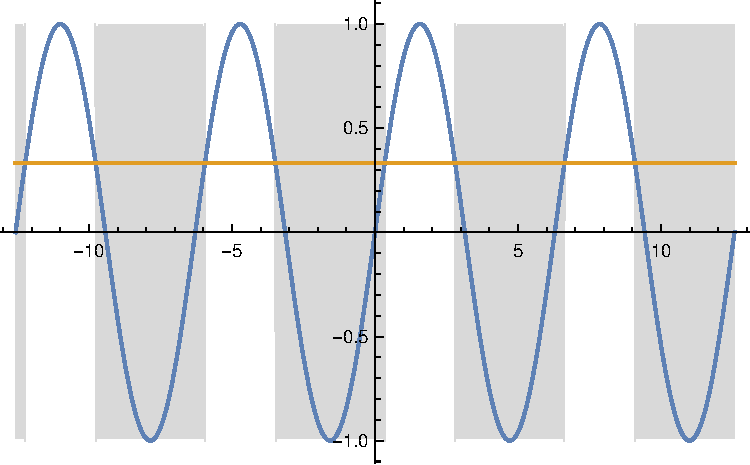
\includegraphics[width=.9\textwidth]{img/interval.pdf}
                \caption{intervals for which \( \sin(X) < y \)}
                \label{interval}
            \end{subfigure}
            \begin{subfigure}{.45\textwidth}
                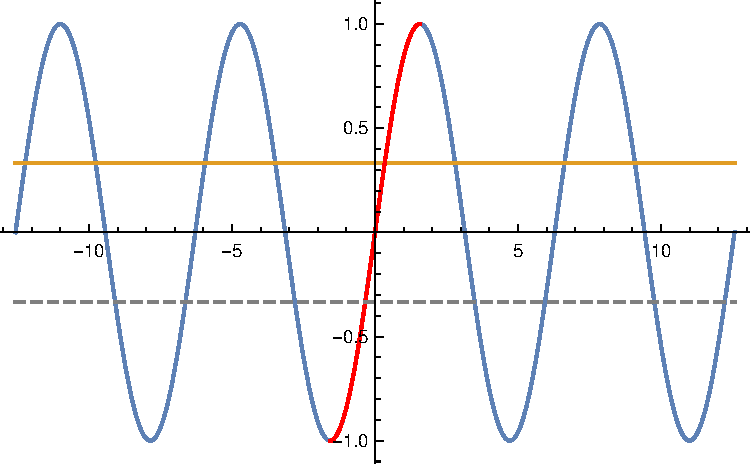
\includegraphics[width=.9\textwidth]{img/inverse.pdf}
                \caption{portion of \( \sin(X) \) which is inverted to get \( \arcsin(X) \) displayed}
                \label{inverse}
        \end{subfigure}
            \caption{Exercise 1.5(c)}
        \end{figure}
 
            Figure \ref{interval} shows the intervals for which \( \sin(X)<y \) is grey, for some \( y \) drawn in orange. Figure \ref{inverse} shows which part of \( \sin \) the inverse is defined on in red. We see that we can find the intervals for which \( \sin(X)<y \) by finding the intersection of \( \sin(X) \) and \( y \) as well as the intersection of \( \sin(X) \) and \( -y \) and then appropriately shifting these endpoints.

        If \( -1<y<1 \) then, \( \sin(X)\leq y \) if and only if for some integer \( k \),
        \begin{align*}
            \arcsin(y)+2k\pi<X<\pi+\arcsin(-y)+2k\pi = \pi-\arcsin(y)+2k\pi
        \end{align*}
        
        Thus, since \( \ZZ \) is countable,
        \begin{align*}
            F_Y(y) &= \PP(\arcsin(y)+2k\pi<X<\pi-\arcsin(y)+2k\pi, \text{for any } k\in\ZZ) \\
                &= \PP\left(x\in\bigvee_{k\in\ZZ}\left( \arcsin(y)+2k\pi<X<\pi-\arcsin(y)+2k\pi \right)\right) \\
                &= \sum_{k\in\ZZ}\PP(\arcsin(y)+2k\pi<X<\pi-\arcsin(y)+2k\pi ) \\
                &= \sum_{k\in\ZZ}\left[F_X(\arcsin(y)+2k\pi)-F_X(\pi-\arcsin(y)+2k\pi)\right]
        \end{align*}

        Therefore, 
        \begin{align*}
            F_Y(y) = 
            \begin{cases} 
                0 & y\leq -1 \\
                \sum_{k\in\ZZ}\left[F_X(\arcsin(y)+2k\pi)-F_X(\pi-\arcsin(y)+2k\pi)\right] & -1<x<1 \\
                1 & y\geq 1
            \end{cases}
        \end{align*}

	\item[(d)]
        Let \( Y=F_X(X) \). We then have,
        \begin{align*}
            F_Y(y) = \PP(Y\leq y) = \PP(F_X(X)\leq y)
        \end{align*}

        Recall \( F_X \) is a (not necessarily strictly) increasing function from \( \RR \) to \( [0,1] \). We deal with this in the following way:
        Define \( g:\RR\to\RR \) by \( g(y) = \sup\{a : F_X(a)\leq y \} \). If \( F_X \) is strictly increasing then \( g(y) = y \) for all \( y \) as desired. Now define \( \hat{F}_X:\RR\to[0,1] \) as \( \hat{F}_X(y) = F_x(g(y)) \). This function is strictly increasing and injective so therefore invertible. Denote the inverse by \( F_X^{-1} \).

Recall \( F_X \) goes from 0 to 1. If \( y<0 \) then \( F_Y(y) = \PP(F_X(X)\leq y < 0) = 0 \). If \( y>1 \) then \( F_Y(y) = \PP(F_X(X)\leq 1<y) = 1 \).

For \( 0<y<a \), we have, 
\begin{align*}
    F_Y(y) = \PP(F_X(X)\leq y) = \PP(X\leq \hat{F}_X^{-1}(y)) = F_X(\hat{F}_X^{-1}(y)) = y
\end{align*}

Thus,
\begin{align*}
    F_Y(y) = 
    \begin{cases}
        0 & y < 0\\ 
        y & 0<y<1 \\
        1 & y>1
    \end{cases}
\end{align*}

Again since the points \( \{0,1\} \) is a set of measure zero it doesn't really matter how we define \( F_Y \) on these points.

\end{enumerate}
\end{solution}

\begin{problem}[Exercise 1.6]
Suppose \( X \) is a continuous random variable defined on a probability space \( (\Omega,\mathcal{F},\mathbb{P}) \). Let \( f \) be the density of \( X \) under \( \mathbb{P} \) and assume \( f>0 \). Let \( g \) be the density function of a random variable. Define \( Z:=g(X)/f(X) \).
\begin{enumerate}
    \item[(a)] Show that \( Z\equiv \text{d}\tilde{\mathbb{P}}/\text{d}\mathbb{P} \) defines a Radon-Nikodym derivative.
	\item[(b)] What is the density of \( X \) under ̃\( \tilde{\mathbb{P}} \)?
\end{enumerate}
\end{problem}

\begin{solution}[Solution]
Suppose \( X \) is a continuous random variable defined on a probability space \( (\Omega,\mathcal{F},\mathbb{P}) \). Let \( f \) be the density of \( X \) under \( \mathbb{P} \) and assume \( f>0 \). Let \( g \) be the density function of a random variable. Define \( Z:=g(X)/f(X) \).
\begin{enumerate}
    \item[(a)] Since \( g \) is a density function, \( g\geq0 \). Thus, \( Z=g(X)/f(X) \geq 0 \). Moreover, since \( g \) is a density, \( \int_\Omega g(x)dx = 1 \). Thus,
        \begin{align*}
            \mathbb{E}Z = \int_\Omega \dfrac{g(x)}{f(x)}f(x)dx = \int_\Omega g(x)dx = 1
        \end{align*}

        Then define \( \tilde{\PP}(A) = \mathbb{E}Z\mathbbm{1}_A \).

        Then \( Z \) is a Radon-Nikodym derivative of \( \tilde{\PP} \) with resepct to \( \PP \).

    \item[(b)] We first compute the distribution of \( X \) under \( \tilde{\PP} \) assuming \( \Omega=\RR \).
        \begin{align*}
            F_X(y) = \tilde{\PP}(X\leq y) = \mathbb{E}Z\mathbbm{1}_{\{X\leq y\}} = \int_\Omega \dfrac{g(x)}{f(x)}\mathbbm{1}_{\{X\leq y\}}f(x)dx = \int_{-\infty}^{y} g(x)dx  
        \end{align*}

        Thus,
        \begin{align*}
            f_X(y) = \dfrac{d}{dy}\int_{-\infty}^{y}g(x)dx = g(y)
        \end{align*}


\end{enumerate}
\end{solution}

\end{document}
